%% The first command in your LaTeX source must be the \documentclass command.
\documentclass[acmtog]{acmart}
\usepackage[english,ngerman]{babel}
\usepackage[utf8]{inputenc}

%% \BibTeX command to typeset BibTeX logo in the docs
\AtBeginDocument{%
  \providecommand\BibTeX{{%
    \normalfont B\kern-0.5em{\scshape i\kern-0.25em b}\kern-0.8em\TeX}}}

% Custom commands for green ticks and red crosses
\usepackage{pifont} % For tick and cross symbols
\definecolor{darkgreen}{RGB}{37, 112, 60}
\newcommand{\cmark}{\textcolor{darkgreen}{\ding{51}}} % Green checkmark
\newcommand{\xmark}{\textcolor{red}{\ding{55}}}   % Red cross

% Command for rotating text 90 degrees
\newcommand*\rot{\rotatebox{90}}

\copyrightyear{2024}
\acmYear{2024}
\citestyle{acmauthoryear}

\usepackage[figurename=Fig.]{caption}
\usepackage{csquotes}
\setcopyright{none}
\makeatletter
\renewcommand{\fnum@figure}{Abb. \thefigure}
\makeatother
\addto\captionsngerman{\renewcommand{\figurename}{Abb.}}
\settopmatter{printacmref=false} % Removes citation information below abstract
\renewcommand\footnotetextcopyrightpermission[1]{} % removes footnote with conference information in first column

\usepackage{minted}

%%
%% end of the preamble, start of the body of the document source.
\begin{document}

%%
%% The "title" command has an optional parameter,
%% allowing the author to define a "short title" to be used in page headers.
\title{Enterprise Architektur-Muster}

%%
%% The "author" command and its associated commands are used to define
%% the authors and their affiliations.
%% Of note is the shared affiliation of the first two authors, and the
%% "authornote" and "authornotemark" commands
%% used to denote shared contribution to the research.
\author{Julian Bruder}
\authornote{Alle Studierenden trugen zu gleichen Teilen zu dieser Arbeit bei.}
\author{Abdellah Filali}
\authornotemark[1]
\author{Luca Franke}
\authornotemark[1]
\affiliation{%
  \institution{Hochschule für Technik, Wirtschaft und Kultur Leipzig (HTWK Leipzig)}
  \streetaddress{Karl-Liebknecht-Str. 132}
  \city{Leipzig}
  \country{Deutschland}
  \postcode{04277}
}
%%
%% By default, the full list of authors will be used in the page
%% headers. Often, this list is too long, and will overlap
%% other information printed in the page headers. This command allows
%% the author to define a more concise list
%% of authors' names for this purpose.
\renewcommand{\shortauthors}{Bruder, Filali, Franke}

%%
%% The abstract is a short summary of the work to be presented in the
%% article.
\begin{abstract}
In diesem Papier werden verschiedene Enterprise Architektur-Muster und deren Rolle in modernen Geschäftsprozessen untersucht
und anschließend unter Einbeziehung technischer und struktureller Eigenschaften anhand ihrer Agilität bewertet.
Dabei orientiert sich die Reihenfolge der Betrachtung jener Architektur-Muster am historischen Verlauf derer Entwicklung und der Notwendigkeit dieser.
Genauer werden die monolithische Architektur, modulare monolithische Architektur, service-orientierte Architektur, Microservice-Architektur, Layered-Architecture,
Event-Driven Architecture, cloud-native Architektur und die Microkernel-Architektur betrachtet.

Insgesamt zeigt sich, dass klassische Enterprise Architektur-Muster zwar mit geringer initialer Komplexität punkten,
mit weiterführender Entwicklung allerdings Flexibilitätsprobleme bedingen.
Dem entgegen zeichnen sich die modernen Architektur-Muster durch hohe Agilität und damit hoher Flexibilität gegenüber den in der modernen Geschäftswelt ständig
wechselnden Anforderungen aus.
Besonders die cloud-native Architektur wird diesen Anforderungen gerecht.
\end{abstract}

\maketitle

\section{Einleitung}
\label{sec:intro}
Moderne Software-Systeme bestehen aus verschiedenen Komponenten \cite{evolutionOfDistributedSystems}.
Dabei nimmt der Nutzer des Systems jenes zwar als eine Software wahr, jedoch verbirgt sich in Realität meist eine Struktur aus
Software-Komponenten und deren Beziehungen hinter dieser Wahrnehmung - ein verteiltes Softwaresystem.
Die Art und Weise dieser Struktur und Beziehungen wird als Architektur bezeichnet.
Wie wird eine solche Architektur mit all ihren Anforderungen der modernen und schnelllebigen Geschäftswelt konstruiert?

Betrachten wir folgend ein Anwendungsbeispiel zur Motivation.
In einem Tech-Startup soll ein Backend für ein internationales E-Commerce-System entwickelt werden.
Dabei werden folgende Anforderungen gestellt:
\begin{itemize}
  \item Zukünftig viele Nutzer und hoher Traffic erwartet
  \item Geringes Kapital für Infrastruktur
  \item Rechtliche Regularien sind teilweise unklar
  \item Hohe Sicherheitsanforderungen aufgrund des Cash-Flows
  \item Agiles Team von acht fähigen Entwicklern
  \item Geldgeber wollen erste Auslieferung in zwei Wochen
\end{itemize}

Das Team arbeitet agil nach Scrum und einigt sich in einer der ersten Planungsphasen auf ein \textit{Minimum Viable Product} (kurz MVP) mit Bestellung, Bezahlung und Versand.
Abbildung \ref{fig:ecommerce-bpm} zeigt die Modellierung des Geschäftsprozesses für diesen MVP\@.
\begin{figure}[!h]
  \centering
  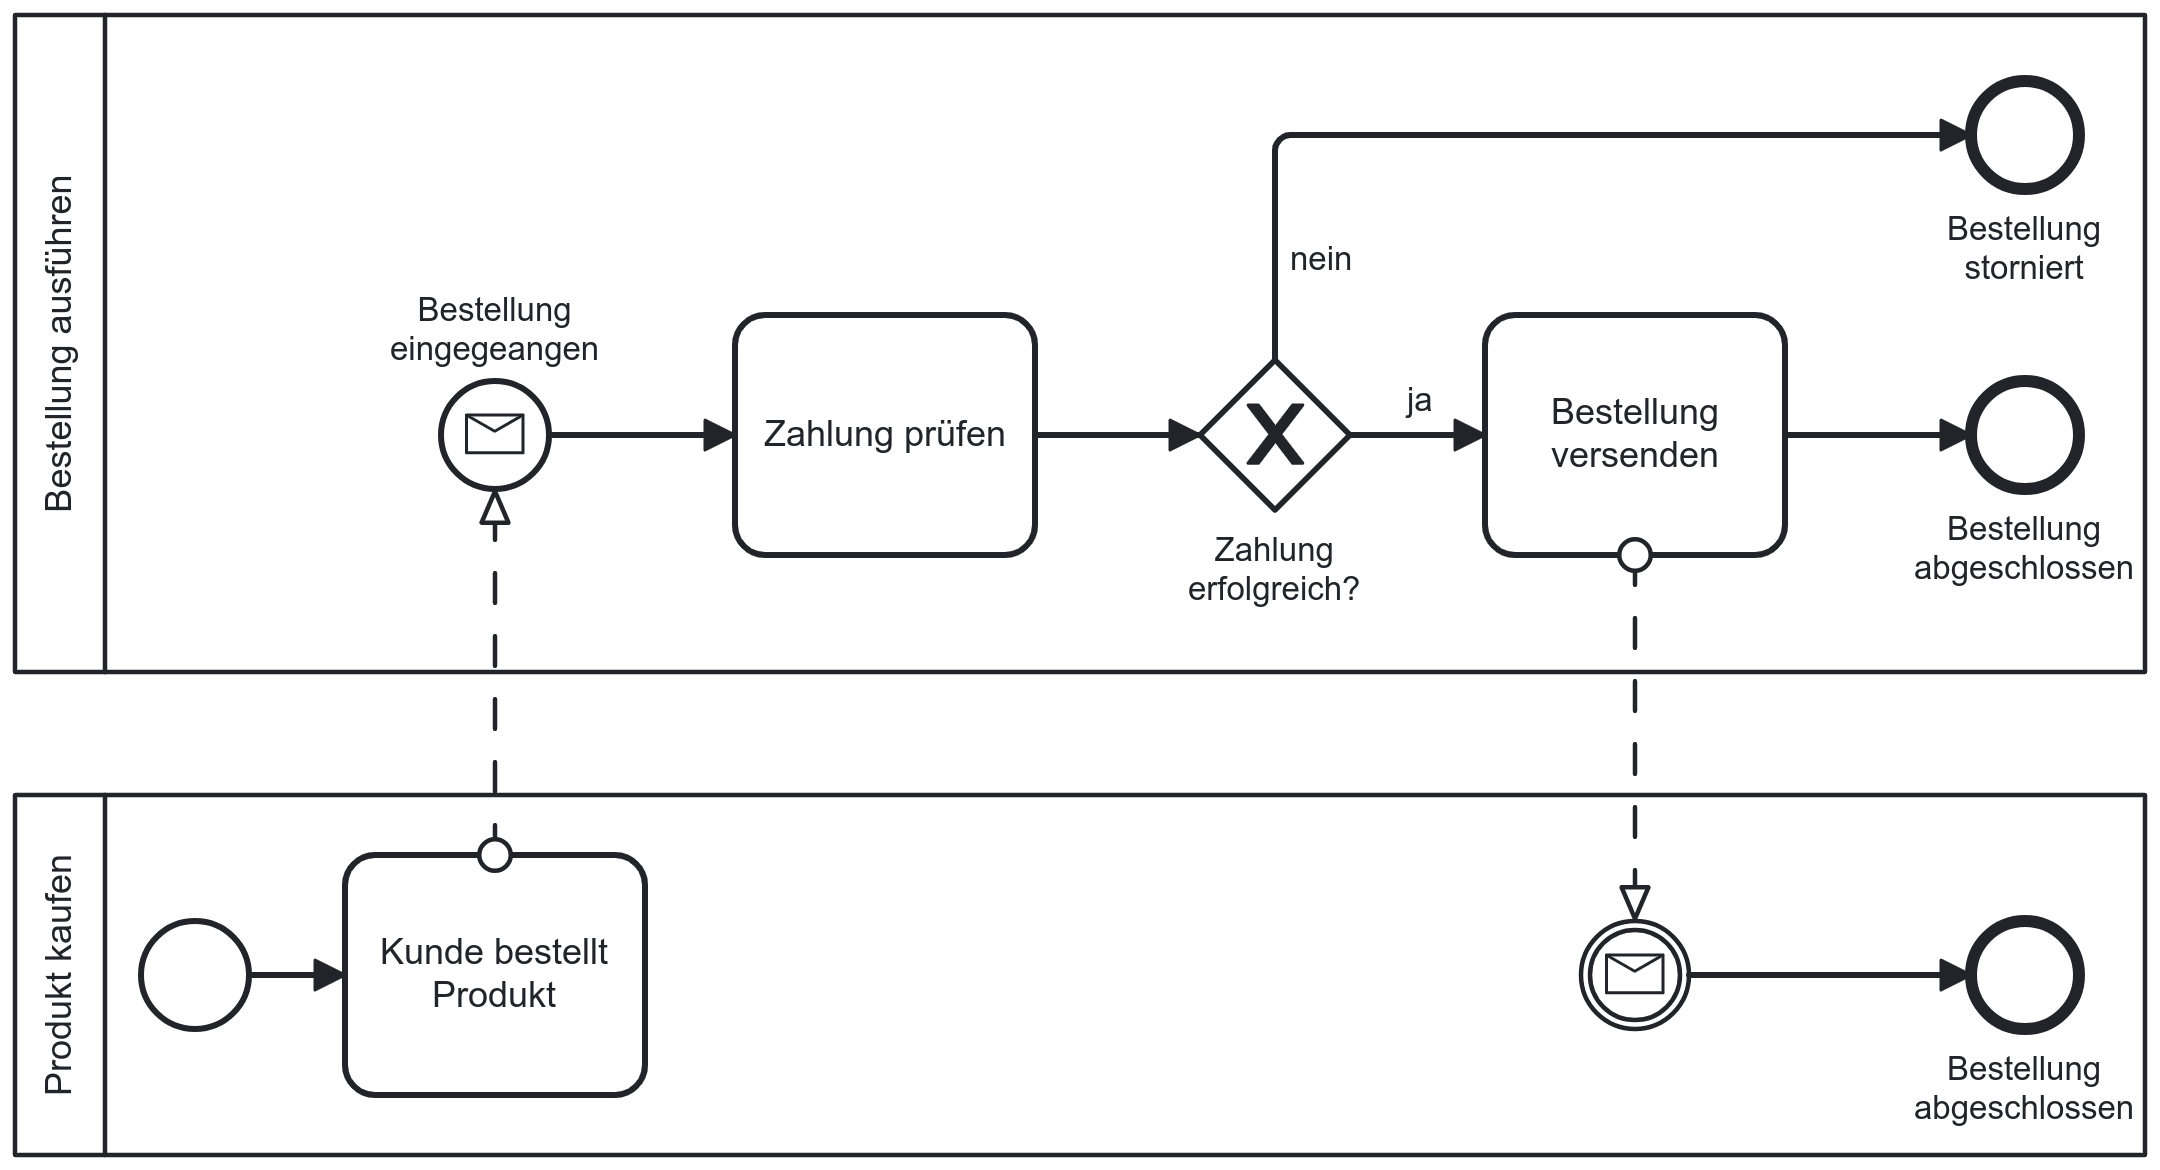
\includegraphics[width=\linewidth]{images/einleitung/ecommerce-order}
  \caption{Geschäftsprozessmodell des MVPs des E-Commerce-Beispiels}
  \label{fig:ecommerce-bpm}
\end{figure}
Die Anforderungen sind somit zwar grob strukturiert aber trotzdem ungewiss.
Die rechtlichen Regularien sind unklar, was zu späten technischen Änderungen führen kann.
Anfangs ist der erwartete Traffic vermutlich niedrig, später sollte dieser aus geschäftlicher Sicht bestenfalls ansteigen.
Wie wird der erwartet hohe Traffic aus infrastruktureller Sicht vorgesehen und finanziert?
Sind acht Entwickler ausreichend?
Kann nach zwei Wochen schon geliefert werden?

All diese Fragen betreffen nicht nur die Software, sondern offensichtlich auch das Geschäft.
Die Antworten dafür liefern Enterprise-Architekturen.
Deren Ziel ist die Ausrichtung von Geschäft und IT, also die Unterstützung des Geschäfts durch die IT und umgekehrt \cite{eaprinciples}.
Ein Enterprise Architektur-Muster ist dabei eine spezifische Strategie zur Umsetzung dieser Ausrichtung.
Erwähnenswert ist hier die Nähe zur Bedeutung des lateinischen Wortes \textit{architectura}.
Wörtlich übersetzt ist es die \textit{Wissenschaft der Baukunst} - meint aber sowohl das Produkt des Bauens als auch den Prozess des Bauens \footnote{https://www.duden.de/rechtschreibung/Architektur, abgerufen am 17.01.2025}.
In Bezug dazu kann die Enterprise-Architektur also als Vision einer grundlegenden Struktur und Beziehungen von Komponenten eines Systems betrachtet werden.
Wichtig ist hierbei die Abgrenzung zur Software-Architektur, der grundlegenden Struktur und Beziehungen von Teilen einer Software.

Im Verlauf der Arbeit werden verschiedene Enterprise Architektur-Muster und deren Rolle in modernen Geschäftsprozessen untersucht
und anschließend unter Einbeziehung technischer und struktureller Eigenschaften anhand ihrer Agilität bewertet.
Dabei wird auch immer auf das eingangs erwähnte und in Abbildung \ref{fig:ecommerce-bpm} dargestellte E-Commerce-Beispiel zurückgegriffen.
Die Arbeit ist wie folgt strukturiert:

Zunächst wird in Abschnitt \ref{sec:monolith} auf die monolithische Architektur eingegangen, bevor die Modularisierung des Monolithen in Abschnitt \ref{sec:modulith} diskutiert wird.
Danach wird in Abschnitt \ref{sec:soa} die service-orientierte Architektur betrachtet.
Folgend wird in Abschnitt \ref{sec:microservices} die Microservice-Architektur diskutiert.
Anschließend wird in Abschnitt \ref{sec:layered} untersucht, wie eine Schichten-Architektur andere, dienst-basierte Architekturen ergänzen kann.
Daraufhin werden sowohl die event-basierte Architektur in Abschnitt \ref{sec:eda} als auch die cloud-native Architektur in Abschnitt \ref{sec:cloudnative} erläutert.
Als letztes Architektur-Muster wird in Abschnitt \ref{sec:microkernel} die Microkernel-Architektur betrachtet.
Abschließend werden die Architekturen in Abschnitt \ref{sec:summary} nach technischen und agilen Kriterien verglichen und folglich die Ergebnisse dieser Arbeit zusammengefasst.

\section{Monolithic Architecture}
\label{sec:monolith}
Der Begriff \textit{Monolith}, abgeleitet aus dem Altgriechischen und mit der Bedeutung
\textit{einheitlicher Stein}\footnote{https://www.duden.de/rechtschreibung/Monolith, abgerufen am 17.01.2025},
wird in der Softwarearchitektur verwendet, um ein Designmuster zu beschreiben, bei dem die gesamte Funktionalität
einer Anwendung in einem einzigen, zusammenhängenden System integriert ist.
In dieser Architektur übernimmt ein einzelner Prozess die Ausführung der gesamten Anwendung \cite[1]{mono}.

Anwendungen, die diesem Architekturansatz folgen, bestehen aus eng miteinander verknüpften
Komponenten, die wechselseitig voneinander abhängen.
Diese Komponenten können weder unabhängig betrieben, noch in bestimmten Fällen,
isoliert kompiliert werden \cite[485]{mono3}.

Diese Architektur bietet insbesondere für kleinere Anwendungen mehrere Vorteile,
wie etwa eine vereinfachte Testbarkeit, Logging, Deployment und Debugging. Ein
weiterer Vorteil besteht darin, dass keine separate Datenbanksynchronisation
erforderlich ist, da sämtliche Daten in einer einzigen Datenbank gespeichert
werden \cite[20358]{mono4}.

Betrachten wir das E-Commerce-Beispiel .
Dafür definieren wir drei Klassen (Siehe Abb. ~\ref{fig:mono}):
\begin{itemize}
  \item \texttt{OrderService}: Klasse, die die Bestellungen verwaltet
  \item \texttt{PaymentService}: Klasse, die die Zahlungen abwickelt
  \item \texttt{ShipmentService}: Klasse, die die Lieferungen initiiert
\end{itemize}

\begin{figure}[h!]
  \centering
  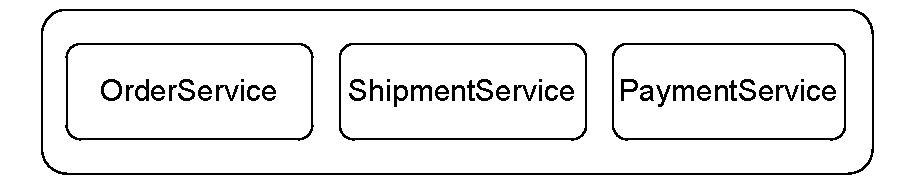
\includegraphics[width=0.4\textwidth]{images/mono/mono.pdf}
  \caption{Monolith Architektur}
  \label{fig:mono}
\end{figure}

Die Kommunikation zwischen den Klassen erfolgt über Methodenaufrufe. In diesem
Zusammenhang stellt die Klasse \texttt{OrderService} die zentrale Komponente dar,
die die Methoden anderer Klassen nutzt, um den Bestellprozess zu steuern. Ein
wesentlicher Vorteil dieses Ansatzes liegt in der einfachen Kommunikation
zwischen den Komponenten.
Durch den direkten Einsatz von Methodenaufrufen
wird die Komplexität verringert, die typischerweise mit der Interaktion zwischen
verschiedenen verteilte Systemen verbunden wäre.

Eine beispielhafte Implementierung des \texttt{PaymentService}s in einer monolithischen
Architektur ist im Anhang \ref{app:code:monolithic:paymentservice} dargestellt.
Der vollständige Quellcode des E-Commerce-Beispiels kann zudem bei GitHub\footnote{https://github.com/Beleg-6-EAP/demo-monolith-ecommerce}
eingesehen werden.

Mit dem Wachstum und der zunehmenden Komplexität der Code-Basis treten jedoch
einige Nachteile auf.
Änderungen an einer Komponente können unerwartete kaskadierende
Fehler auslösen, was die Weiterentwicklung in kleinen, autonomen Teams erschwert
und verlangsamt.

Ein weiterer Nachteil ergibt sich aus der engen Kopplung zwischen den Komponenten,
die durch direkte Methodenaufrufe entsteht.
Änderungen an der Implementierung oder
der Signatur einer Methode können in der Folge die gesamte Anwendung beeinflussen.

Zudem wird die Wiederverwendung von Funktionalitäten erschwert, da die Komponenten
stark miteinander verknüpft sind.
Dies führt zu einer Duplizierung von Code, was die Kosten für Änderungen erhöht,
da diese an mehreren Stellen vorgenommen werden müssen.

Die daraus resultierende Komplexität und die erschwerte Wartung führen zu längeren
Iterationen.
Da das Deployment nur als Ganzes erfolgen kann und die Iterationen
sich verlängern, kommt es zu seltenen Auslieferungen.

Ein weiteres Problem liegt in der erschwerten horizontalen Skalierung, da die Anwendung
nur als Ganzes skaliert werden kann.
Dies stellt eine Herausforderung dar, da bei wachsenden
Anforderungen die gesamte Anwendung skaliert werden muss, anstatt einzelne Komponenten unabhängig
voneinander zu skalieren.

Insgesamt ist die monolithische Architektur eine geeignete Lösung für
kleinere Anwendungen, jedoch weniger geeignet für größere Systeme, da sie die Agilität und
Flexibilität erheblich einschränken kann.

\section{Modular Monolithic Architecture}
\label{sec:modulith}
Das Hauptproblem der zuvor beschriebenen Architektur liegt in der engen Kopplung der Komponenten,
was zu einer erhöhten Komplexität und begrenzten Flexibilität führt.
Die Modular Monolithic Architecture stellt eine Weiterentwicklung der Monolithic Architecture dar,
indem sie die Vorteile des monolithischen Ansatzes bewahrt und gleichzeitig die Nachteile
der engen Kopplung verringert.

In diesem Architekturmodell wird die Code-Basis in mehrere Module unterteilt, die jeweils
eine spezifische Teilfunktionalität der Anwendung implementieren.\cite[11]{modular-mono2}.

Die Modularisierung trägt zudem zur Reduzierung der Komplexität bei und ermöglicht eine bessere
Organisation der Code-Basis, was sich positiv auf die Wartbarkeit der Anwendung auswirkt \cite[23 - 24]{modular-mono4}.


Betrachten wir erneut das E-Commerce-Beispiel.
Diesmal wird die Anwendung in drei Hauptmodule aufgeteilt (Siehe Abb. ~\ref{fig:modular-mono}):
\begin{itemize}
  \item \texttt{order}: Modul, das für die Verwaltung der Bestellungen verantwortlich ist
  \item \texttt{payment}: Modul, das für die Abwicklung der Zahlungen verantwortlich ist
  \item \texttt{shipment}: Modul, das für die Initiierung der Lieferungen verantwortlich ist
\end{itemize}

\begin{figure}[h!]
  \centering
  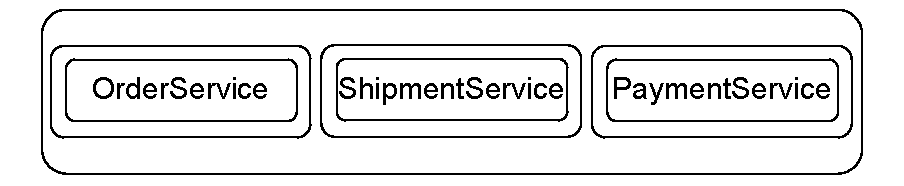
\includegraphics[width=0.4\textwidth]{images/mono/mono-example.pdf}
  \caption{Modular Monolith Architektur}
  \label{fig:modular-mono}
\end{figure}

Wie Abbildung \ref{fig:modular-mono} zeigt, ist jeder Service in einem eigenen Modul gekapselt.
Ein konkretes Beispiel hierfür bietet die Implementierung des \texttt{OrderService}s, welche im Modul \texttt{order}
realisiert ist (siehe Anhang \ref{app:code:modular:orderservice}). Die Logik des \texttt{OrderService} ist vollständig
innerhalb des entsprechenden Moduls integriert, während die Kommunikation mit anderen Modulen durch klar definierte
Spezifikationen geregelt wird.
Für weiterführende Informationen und die vollständige Implementierung des E-Commerce-Beispiels
wird auf das GitHub-Repository verwiesen\footnote{https://github.com/Beleg-6-EAP/demo-modulith-ecommerce}.

Durch die Modularisierung sind die Komponenten weniger eng miteinander gekoppelt, was eine
verbesserte Zusammenarbeit in kleinen, autonomen Teams fördert, im Vergleich zu traditionellen
monolithischen Ansätzen.

Ein Nachteil bleibt jedoch bestehen: Die Anwendung muss weiterhin als Ganzes deployed werden,
was die Iterationen verlangsamt.
Zudem bleibt die horizontale Skalierung weiterhin erschwert,
und die Funktionalitäten können nicht wiederverwendet werden, da sie immer noch Teil einer
einzigen Anwendung sind und eng miteinander gekoppelt bleiben.

\section{Service-oriented Architecture}
\label{sec:soa}
Bei der (modularen) monolithischen Architektur zeigte sich die enge Kopplung der Funktionalitäten als zentrales Problem.
Dieses Problem löst die service-orientierte Architektur (kurz SOA), indem sie den Fokus auf die Nutzung wiederverwendbarer Dienste (englisch \textit{services}) setzt.
Ein Dienst ist dabei eine meist grob-granulare Unternehmensfunktionalität.

Betrachten wir im Folgenden die Komponenten einer SOA:
\begin{itemize}
  \item Service Provider: Komponente, die einen spezifischen Dienst anbietet \cite{soa4}
  \item Service Consumer: Komponente, die einen bereitgestellten Dienst nutzt
  \item Service Registry: Komponente zur Sammlung von Metadaten über Dienste
  \item Service Bus: Zentrale Komponente, die sowohl als Broker zwischen Providern und Konsumenten fungiert als auch zusätzliche Aufgaben wie beispielsweise Routing übernimmt
\end{itemize}

Die Beziehungen zwischen diesen Komponenten sind in Abbildung \ref{fig:soa} dargestellt.
\begin{figure}[!h]
  \centering
  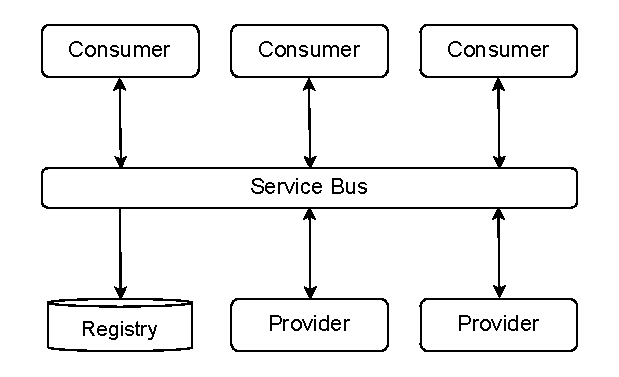
\includegraphics[width=0.8\linewidth]{images/soa/soa.pdf}
  \caption{Aufbau der Service-oriented Architecture}
  \label{fig:soa}
\end{figure}
Darin ist zu erkennen, dass Provider und Consumer sich nicht gegenseitig kennen.
Damit ein Consumer trotzdem einen Dienst eines Providers nutzen kann, werden Metadaten zum Provider und dessen Dienst in einer Service-Registry gespeichert.
Durch diese kann der Service-Bus auf Anfrage eines Consumers für einen spezifischen Dienst einen solchen in der Service-Registry suchen.
Wenn ein solcher dort gelistet ist, dann kann der Consumer den Dienst des Providers per Kommunikation über den Service-Bus nutzen.
Damit dient dieser offensichtlich als Vermittler zwischen Consumer und Provider, wobei der Consumer die Spezifikation einer Unternehmensfunktionalität nutzt,
der Provider diese implementiert und die Registry jene persistiert \cite[16]{soa2}\cite[19-26]{soa4}.
Daher sind Provider und Consumer lose zueinander gekoppelt.
Um die Kommunikation am Bus zu vereinheitlichen, wird auf standardisierte Web-Kommunikation zurückgegriffen.
Meist werden dafür zum Nachrichtenaustausch das Protokoll SOAP und die Schnittstellenbeschreibungssprache WSDL verwendet. % TODO: Quelle!!!

Betrachten wir im Folgenden die Anwendung einer SOA auf das E-Commerce-Beispiel.
Dafür definieren wir drei verschiedene Services:
\begin{itemize}
  \item \texttt{OrderService}: Ein Dienst, der den gesamten Bestellvorgang verwaltet
  \item \texttt{PaymentService}: Ein Dienst, der den gesamten Bezahlvorgang verwaltet
  \item \texttt{ShipmentService}: Ein Dienst, der den gesamten Versandvorgang verwaltet
\end{itemize}

Abbildung \ref{fig:soaecommerce} stellt die Anwendung der Architektur auf das Beispiel dar.
\begin{figure}[!h]
  \centering
  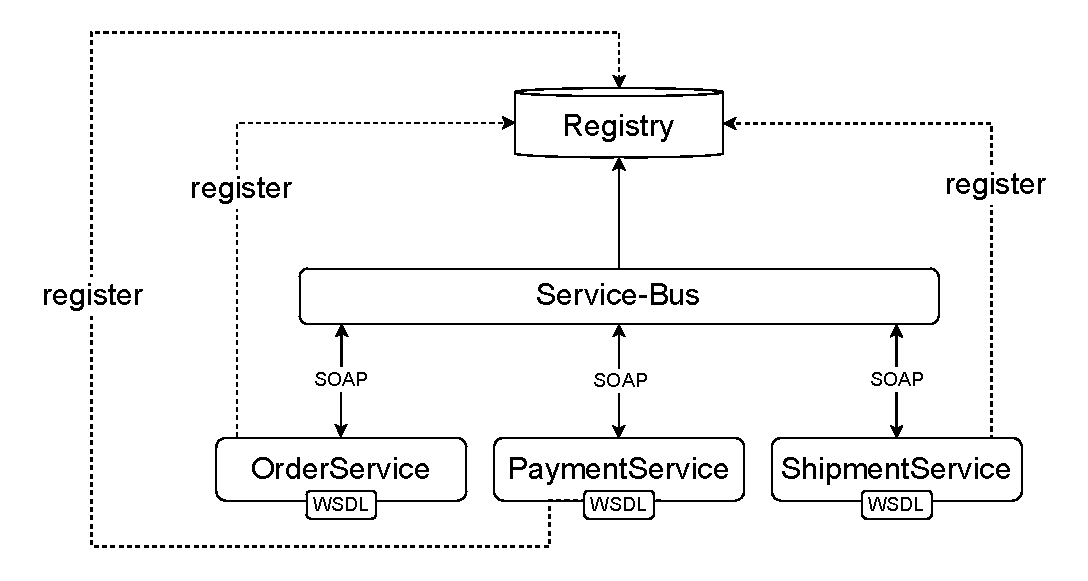
\includegraphics[width=0.8\linewidth]{images/soa/soa-example.pdf}
  \caption{E-Commerce-Beispiel mit Service-oriented Architecture}
  \label{fig:soaecommerce}
\end{figure}

Alle drei Dienste agieren dabei offensichtlich als Provider und registrieren ihre Dienste bei der Registry.
Der \texttt{OrderService} nutzt die Spezifikation der beiden Dienste für Bezahlung und Versand, ist also zusätzlich Konsument.
Die Konsumierung der Dienste erfolgt dabei sequenziell, indem der \texttt{OrderService} nach Lokalisierung von \texttt{PaymentService} und \texttt{ShipmentService}
erst mit ersterem und dann mit letzterem über den Bus via SOAP kommuniziert.

Da die Provider ihre Dienste dabei mit WSDL spezifizieren und die Registry diese speichert, können die Implementierungen leicht ausgetauscht werden.
Im Beispiel könnte dabei möglicherweise ein spezifischer \texttt{PaymentService} von PayPal durch einen von Apple Pay ersetzt werden.
Wenn sich die Spezifikation jener nicht ändert, dann ändert sich auch die Nutzung der Funktionalität beim Consumer nicht, sodass dieser einfach
auf geänderte Anforderungen reagieren kann.

Im Anhang \ref{app:code:soa:registry} ist eine beispielhafte Implementierung der Service-Registry zu finden.
Die vollständige Implementierung des E-Commerce-Beispiels kann bei GitHub\footnote{https://github.com/Beleg-6-EAP/demo-soa-ecommerce} eingesehen werden.

Wie schon bei der modularen Monolithen-Architektur in Abschnitt TODO ermöglicht die lose Kopplung kleine autonome Teams.
Im Gegensatz zu jener Architektur können aufgrund der Eigenständigkeit der Services in einer SOA jene allerdings auch individuell pro Team ausgeliefert werden.
Das ermöglicht kürzere Iterationen und somit häufigere Auslieferung als beim modularen Monolithen.
Dadurch und durch die lose Kopplung kann außerdem flexibler auf wechselnde Anforderungen reagiert werden.
Ebenfalls können Entwicklungszeit gesenkt und somit auch Kosten durch die Wiederverwendbarkeit von Diensten eingespart werden werden.

Die meist grobe Granularität der Dienste führt allerdings langfristig zu Abhängigkeiten zwischen Diensten.
Aus diesem Grund und der zentralen Abhängigkeit der Dienste an den Service-Bus lassen sich Systeme mit SOA jedoch weiterhin schwer horizontal skalieren.

\section{Microservices Architecture}
\label{sec:microservices}
Die Microservices Architecture greift grundlegend das Konzept einer Service-oriented Architecture auf, legt den Fokus aber auf eine fein granuliertere Aufteilung mit dem Ziel der Isolation.

Die bisher meist grob granulierten Dienste werden auf einzelne Funktionalitäten reduziert und bestenfalls vollständig voneinander isoliert.
Im Gegensatz zu SOA greifen die Services nicht mehr auf eine zentrale Persistenz-Schicht zu, sondern haben private, für andere nicht einsehbare Persistenzen\cite[2]{microservicesArchitecture}.

Wie in Abbildung~\ref{fig:microservices} dargestellt, werden alle von Clients ausgehenden API-Anfragen zunächst von einem API-Gateway entgegengenommen.
Da Anfragen von Clients oft mehrere Services betreffen, wird das Gateway als Vermittler genutzt, um die Anfragen an die entsprechenden Services zu orchestrieren.
Dabei profitiert das Gateway von geringen Latenzen aufgrund von physikalischer Nähe zu den Service Komponenten und einer besseren Netzwerkanbindung im Vergleich zum Client.
Bei Anfragen an mehrere Services akkumulieren sich diese Ersparnisse und Antwortzeit verkürzt sich insgesamt~\cite[30]{architecturePatterns}.
Da Gateways keine Daten halten, sondern nur Anfragen weiterleiten, sind sie leicht horizontal skalierbar und können bei Bedarf um weitere Instanzen erweitert werden.

\begin{figure}[!h]
  \centering
  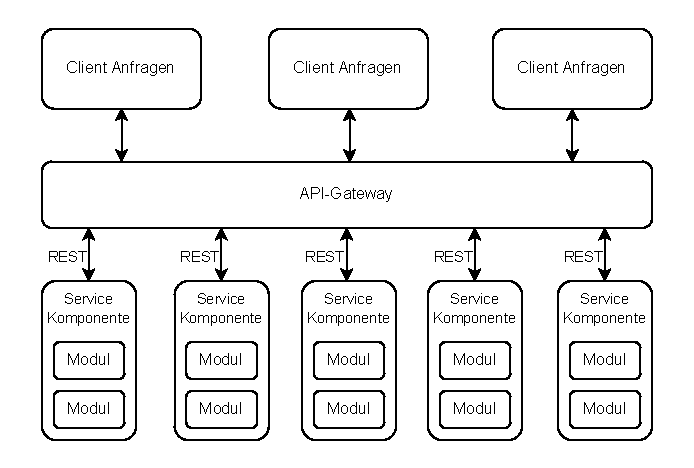
\includegraphics[width=\linewidth]{images/microservices/microservices}
  \caption{Aufbau einer Microservices Architecture}
  \label{fig:microservices}
\end{figure}

Es besteht die Möglichkeit die Service-Komponenten mit unterschiedlichen Technologien zu entwickeln, da die Kommunikation über standardisierte Schnittstellen stattfindet.
Diese Schnittstellen sind meist REST-Endpunkte, können aber mithilfe von alternativen Protokollen wie Messaging Queues, RPC oder Event-Streaming implementiert sein.
Durch die Aufteilung in isolierte Komponenten, kann die Entwicklung dieser auf kleine, autonome Teams verteilt werden.

Damit ist die Entkopplung der einzelnen Services ein maßgebendes Merkmal dieses Musters.
Dies wird dadurch erreicht, dass alle Services nur über ihre definierten Schnittstellen, miteinander kommunizieren können.
Die hohe Entkopplung der Komponenten ermöglicht es, Services unabhängig voneinander zu entwickeln, zu testen und auszuliefern.
Pipeline- und Deploymentprozesse finden also ebenfalls isoliert voneinander statt, was die Auslieferung der Software beschleunigt~\cite[27]{architecturePatterns}.

Der korrekte Entwurf der Architektur und die darin passend gewählte Granularität der Services ist entscheidend, um die Vorteile der Microservices Architecture voll auszuschöpfen und stellt hier die größte Herausforderung dar.
Werden die Komponenten zu groß gewählt, dann könnten die Vorteile der Microservices Architecture nicht mehr greifen, weil innerhalb der Komponenten Abhängigkeiten entstehen, die das isolierte Entwickeln oder Testen von Features verhindern.
Auf der anderen Seite führt eine zu geringe Granularität dazu, dass die Anzahl der Services zu groß wird und die Kommunikation einen zu großen Overhead verursacht.
Jede Nachricht, die unter den Services ausgetauscht wird, verursacht Latenz, die sich akkumuliert und die Performance des Systems beeinträchtigt.
Weiterhin werden Integrationstests durch die hohe Anzahl an Services aufwändiger und der Orchestrierungsaufwand des Gateways steigt an~\cite[32]{architecturePatterns}.

Sollten serviceübergreifende Persistenz-Zugriffe notwendig sein, so könnten diese über eine geteilte Datenbank stattfinden.
Dadurch werden ungewollte Abhängigkeiten zwischen Services vermieden und die Kopplung der Komponenten verringert.
Dabei ist jedoch darauf zu achten, dass die Datenbank nicht zu einer zentralen Abhängigkeit wird, die die Vorteile der Microservices Architecture wieder rückgängig macht~\cite[33]{architecturePatterns}.

\begin{figure}[!h]
  \centering
  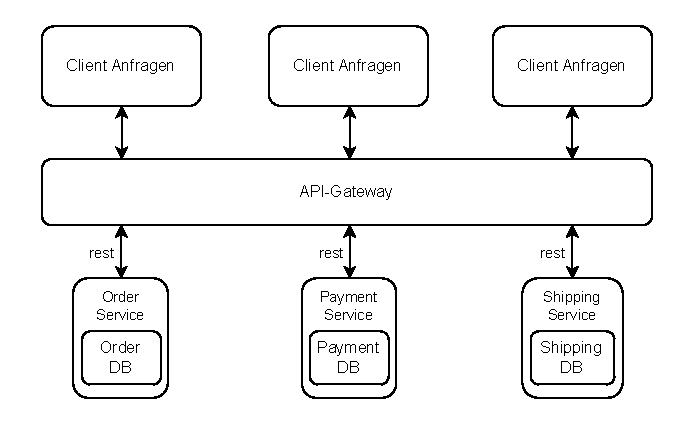
\includegraphics[width=\linewidth]{images/microservices/ecommerce-microservices}
  \caption{Aufbau der E-Commerce Anwendung mit Microservices Architecture}
  \label{fig:ecommerce-microservices}
\end{figure}

Betrachten wir nun, wie dieses Architekturmuster auf das Beispiel der E-Commerce Anwendung übertragen werden kann.
Ein möglicher Aufbau der Anwendung ist in Abbildung~\ref{fig:ecommerce-microservices} dargestellt.
Sie ist in drei Services aufgeteilt, die jeweils für die Verarbeitung von Bestellungen, Zahlungen und Versand verantwortlich sind.
Jeder Service hat seine eigene Datenbank und REST-Schnittstelle, über die er mit anderen Services und dem Gateway kommuniziert.
Änderungen am Bezahl- oder Versandprozess können so unabhängig vom eigentlichen Bestellprozess entwickelt und ausgeliefert werden.
Auch besteht die Möglichkeit bei besonders hohen Lasten oder Engpässen, die Services unabhängig voneinander horizontal zu skalieren.

Die Microservices Architecture löst viele der Probleme, die in klassischen monolithischen oder Service-oriented Architecture auftreten.
Durch die Aufteilung der Anwendung in kleinere, separat ausgelieferte Services, entstehen inhärent robustere und besser skalierbare Systeme.
Da Änderungen oft nur einzelne Service Komponenten betreffen, muss nicht das ganze System neu ausgeliefert werden.
Es reicht stattdessen, nur den betroffenen Service zu aktualisieren, was die Ausfallzeiten minimiert und die Wartbarkeit der Software erhöht.
Vor allem in agilen Umgebungen, in denen viele Iterationen und schnelle Auslieferungen notwendig sind, ist die Microservices Architektur daher besonders geeignet~\cite[33]{architecturePatterns}.

Auch können Services in produktiven Umgebungen ohne Ausfallzeiten ausgetauscht werden.
Solange, wie der neue Service ausgeliefert wird, leitet das API-Gateway Anfragen an den alten Service weiter.
Erst wenn der neue Service bereit ist, werden Anfragen an diesen weitergeleitet und der alte Service kann abgeschaltet werden.

Microservices sind außerdem sehr gut testbar.
Tests können durch die strikte Trennung der Funktionalitäten isoliert auf einzelne Services angewendet werden, ohne dass andere Services betrachtet werden müssen.
Auch Regressionstests nehmen dadurch weniger Zeit in Anspruch.
Kleine Änderungen haben nicht zur Folge, dass die gesamte Anwendung neu getestet werden muss.

Obwohl die Auslieferungen schnell sind und parallel an verschiedenen Services gearbeitet werden kann, ist die initiale Entwicklungszeit einer Anwendung in Microservices Architecture oft groß.
Im Vergleich zu monolithischen Anwendungen ist vor allem mit höherem Zeitaufwand durch Entwurf der Schnittstellen, Absprache unter den Entwicklungsteams und Planung der Architektur zu rechnen~\cite[6-7]{evolutionOfDistributedSystems}.

Der größte Nachteil der sich hier ergibt, ist die vergleichsweise niedrige Performance aufgrund der verteilten Natur des Systems.
Die Kommunikation zwischen Services findet meist über das Netzwerk statt, was zu erhöhten Latenzen führen kann\cite[34]{architecturePatterns}.

\section{Layered-Architecture}
\label{sec:layered}
Das Problem der redundanten Schnittstellenlogik in Microservices lässt sich durch die
Anwendung der Layered Architecture effektiv lösen. Dieses Architekturmuster basiert auf
der Grundidee, eine Anwendung in verschiedene Schichten (englisch \textit{layers})
zu gliedern. Dabei bleiben sowohl die Anzahl der Schichten als auch deren spezifischen
Aufgaben flexibel und werden nicht durch das Muster vorgeschrieben \cite[34]{layered2}.

Diese Flexibilität erlaubt es Unternehmen, die Schichtstruktur individuell an ihre
spezifischen Anforderungen anzupassen. Um jedoch Vorteile wie eine verbesserte Wartbarkeit,
Skalierbarkeit und Wiederverwendbarkeit zu realisieren, ist die Einhaltung zentraler
Prinzipien der Layered Architecture essenziell \cite[34]{layered2}.

Ein grundlegendes Prinzip ist die Trennung der Zuständigkeiten (englisch \textit{Separation
of Concerns}). Hierbei werden Komponenten mit unterschiedlichen Aufgaben in separate Schichten
aufgeteilt, sodass jede Schicht ausschließlich für eine klar definierte und abgeschlossene
Funktionalität verantwortlich ist \cite[34]{layered2}.

Ein weiteres wesentliches Prinzip ist die Isolation der Schichten (englisch \textit{Layers
of Isolation}), welches gewährleistet, dass Änderungen innerhalb einer Schicht lediglich
deren eigene Komponenten betreffen und keine Auswirkungen auf andere Schichten haben \cite[3–4]{architecturePatterns}.

Die Layered Architecture bietet insbesondere für Unternehmen die Möglichkeit, häufig genutzte
Funktionalitäten, wie etwa Authentifizierung oder Logging, in dedizierten Schichten zu kapseln
und diese flexibel in verschiedenen Diensten wiederzuverwenden. Dabei sorgt eine klar definierte
Schnittstelle jeder Schicht sowohl für eine reibungslose Kommunikation als auch für die
Abstraktion der internen Implementierung.

Zusätzlich lässt sich die Layered Architecture nahtlos mit modernen agilen Architekturmustern
wie Microservices kombinieren, wodurch die Agilität eines Unternehmens weiter gesteigert werden
kann.

Ein praxisnahes Beispiel hierfür ist das E-Commerce-Beispiel mit Microservices.
In der ursprünglichen Implementierung enthielt jeder Service ein eigenes Modul für die Authentifizierung. Diese
redundante Struktur führte jedoch zu erheblichen Herausforderungen hinsichtlich Wartbarkeit
und Kosten: Änderungen an der Authentifizierungslogik mussten in jedem einzelnen Service separat
durchgeführt werden, was den Entwicklungsprozess verlangsamte und unnötig komplizierte.

Eine Lösung für dieses Problem besteht darin, die Authentifizierungslogik in eine zentrale
Schicht auszulagern.
Diese Schicht kann direkt mit dem API-Gateway kommunizieren
und somit eine einheitliche Authentifizierung gewährleisten (siehe Abb. ~\ref{fig:layered}).

\begin{figure}[h!]
  \centering
  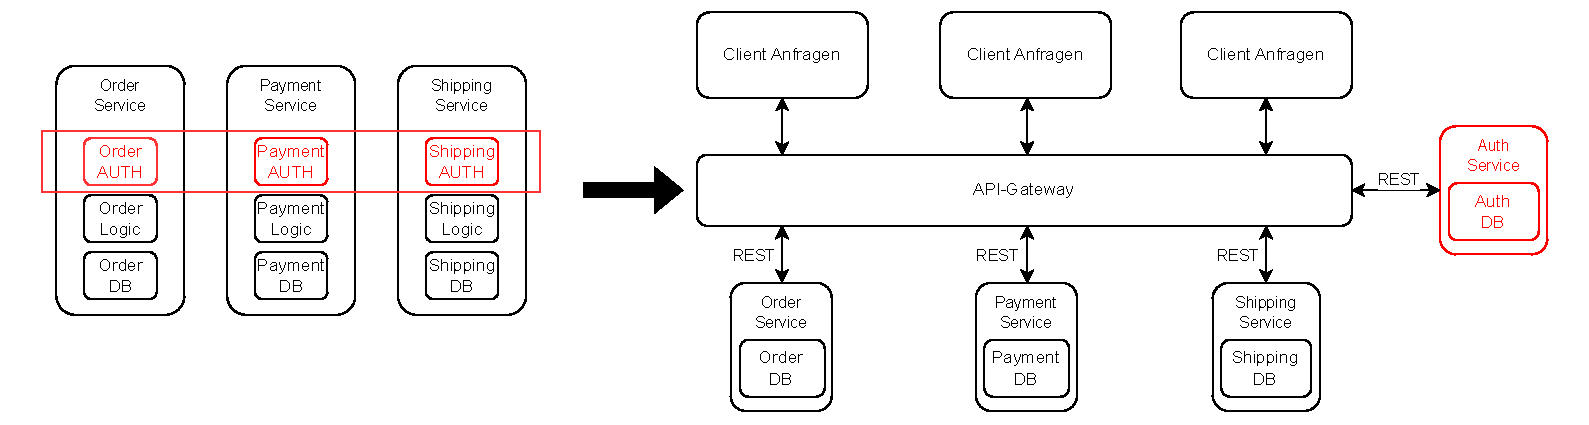
\includegraphics[width=0.5\textwidth]{images/layered/ecommerce-example}
  \caption{Layered Microservice Architecture: Beispiel E-Commerce}
  \label{fig:layered}
\end{figure}

Mit der Einführung einer zentralen Authentifizierungsschicht kann die Authentifizierungslogik
an einer einzigen Stelle gebündelt und bei Bedarf angepasst werden, ohne Änderungen in den
einzelnen Services vornehmen zu müssen.
Dies bietet insbesondere in Unternehmen mit einer Vielzahl von Services signifikante Zeit- und Kosteneinsparungen.

Ein weiterer Vorteil besteht darin, dass die Authentifizierung für sämtliche Dienste
zentral über ein API-Gateway durchgeführt wird, wodurch eine wiederholte Authentifizierung
auf Service-Ebene entfällt.
Diese Entlastung erlaubt es den einzelnen Services, sich ausschließlich auf ihre
Kernfunktionalität zu konzentrieren, während die Authentifizierung ausgelagert ist.

Die vollständige Implementierung des E-Commerce-Beispiels mit geschichteter Microservice-Architektur
ist bei GitHub \footnote{https://github.com/Beleg-6-EAP/demo-microservice-ecommerce} zu finden.

Die klare Trennung der Verantwortlichkeiten fördert die Zusammenarbeit in kleinen, autonomen
Teams, da jedes Team unabhängig an einer Schicht arbeiten kann.
Zudem ermöglicht das Prinzip der Isolation der Schichten eine höhere Flexibilität gegenüber wechselnden Anforderungen.
Durch die Wiederverwendbarkeit in der Layered Architecture wird Mehraufwand vermieden und duplizierter
Code reduziert, was zu kürzeren Iterationen und häufigeren Auslieferungen führt.

Das Beispiel verdeutlicht zudem, dass die Layered Architecture sich hervorragend mit agilen
Architekturen wie Microservices kombinieren lässt.
Diese Synergie trägt entscheidend dazu bei, die Agilität des Systems nachhaltig zu steigern.

\section{Event-Driven Architecture}
\label{sec:eda}
Die Event-Driven Architecture wählt als Basis einen anderen Ausgangspunkt als die bisherigen Architekturmuster.
Während bei letzteren Komponenten Dienste bereitstellen, welche von anderen Komponenten explizit genutzt werden,
verhalten sich Dienst-bereitstellende Komponenten in der Event-Driven Architecture reaktiv,
werden also implizit von Dienst-konsumierenden Komponenten genutzt \cite{garlanShawImplizit}.
Ein System reagiert somit asynchron auf Zustandsänderungen, also Ereignisse in diesem System \cite{eda}.
Die in dieser Architektur minimalen Einheiten, welche Informationen einer Zustandsänderung kapseln, werden \textit{Events} genannt.
Die Idee der impliziten Behandlung von Ereignissen ist nicht neu und taucht erstmals 1994 im von Garlan und Shaw publizierten Papier
\textit{\enquote{An introduction to Software Architecture}} auf.

Betrachten wir im Folgenden die Basis-Bestandteile der Event-Driven Architecture:
\begin{itemize}
  \item Ereignis (englisch \textit{Event}): Kapselt Information einer Zustandsänderung eines Systems
  \item Produzent (englisch \textit{Producer}): Komponente, die Event erzeugt
  \item Herausgeber (englisch \textit{Publisher}): Komponente, die, von Produzenten erzeugte, Events publiziert
  \item Konsument (englisch \textit{Consumer}): Komponente, die auf publizierte Events reagiert
  \item Vermittler (englisch \textit{Mediator}): Komponente zwischen Produzenten und Konsumenten - filtert Events und verteilt diese auf Konsumenten
  \item Event-Bus: Oft auch \textit{Event-Broker} genannt - bietet die Infrastruktur für die Gesamtheit der Vermittler
\end{itemize}
Abstrakt kann ein Event als Vertrag zwischen Produzenten und Konsumenten am Event-Bus betrachtet werden.
Der Konsument nutzt die Spezifikation des Events am Bus, der Produzent implementiert jene Spezifikation.
Abbildung \ref{fig:eda} stellt diesen Vertrag dar.

\begin{figure}[!h]
  \centering
  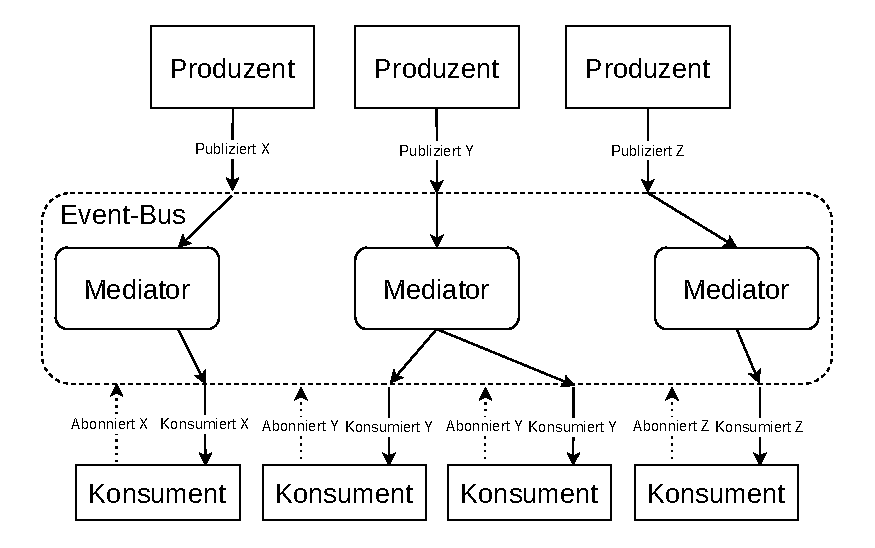
\includegraphics[width=\linewidth]{images/eda/eda.drawio}
  \caption{Vertrag zwischen Produzenten und Konsumenten am Event-Bus}
  \label{fig:eda}
\end{figure}

Durch den Vertrag weisen die Events am Event-Bus starke Kohäsion und somit lose Kopplung auf.
Diese lose Kopplung minimiert nicht nur kaskadierende Fehler, sondern ermöglicht kleinen und autonomen Entwickler-Teams
die klare Abgrenzung von Features und folglich einfach definierbare Iterationen - eine Menge von Events, deren Erzeugung und Konsumierung.

Weiter sind Events oft nah an dem, was Ereignisse in realen Prozessen sind, also domain-driven.
Gebündelt ermöglichen obige Punkte die kontinuierliche Auslieferung von Software in kurzen Intervallen.

Außerdem garantiert die asynchrone Behandlung von Ereignissen zusammen mit der loosen Kopplung hohe Skalierung und die Möglichkeit für Echtzeit-Software.
Daher sind Event-Driven Architekturen besonders für datenintensive Echtzeit-Anwendungen wie IoT (Internet of Things) und Analytics geeignet \cite{iotEda}.

Betrachten wir erneut das E-Commerce-Beispiel aus der Einleitung.
Dafür definieren wir drei Arten von Events:
\begin{itemize}
  \item \texttt{OrderCreated}: Ein Event, das genau dann erzeugt wird, wenn eine neue Bestellung aufgegeben wird
  \item \texttt{PaymentProcessed}: Ein Event, das genau dann erzeugt wird, wenn der Bezahlvorgang abgeschlossen wird
  \item \texttt{ShipmentInitiated}: Ein Event, das genau dann erzeugt wird, wenn die Bestellung versandt wird
\end{itemize}

Analog zur Microservice-Architektur teilen wir die Funktionalitäten in drei verschiedene Dienste auf: \texttt{OrderService}, \texttt{PaymentService} und \texttt{ShipmentService}.

\begin{figure}[!h]
  \centering
  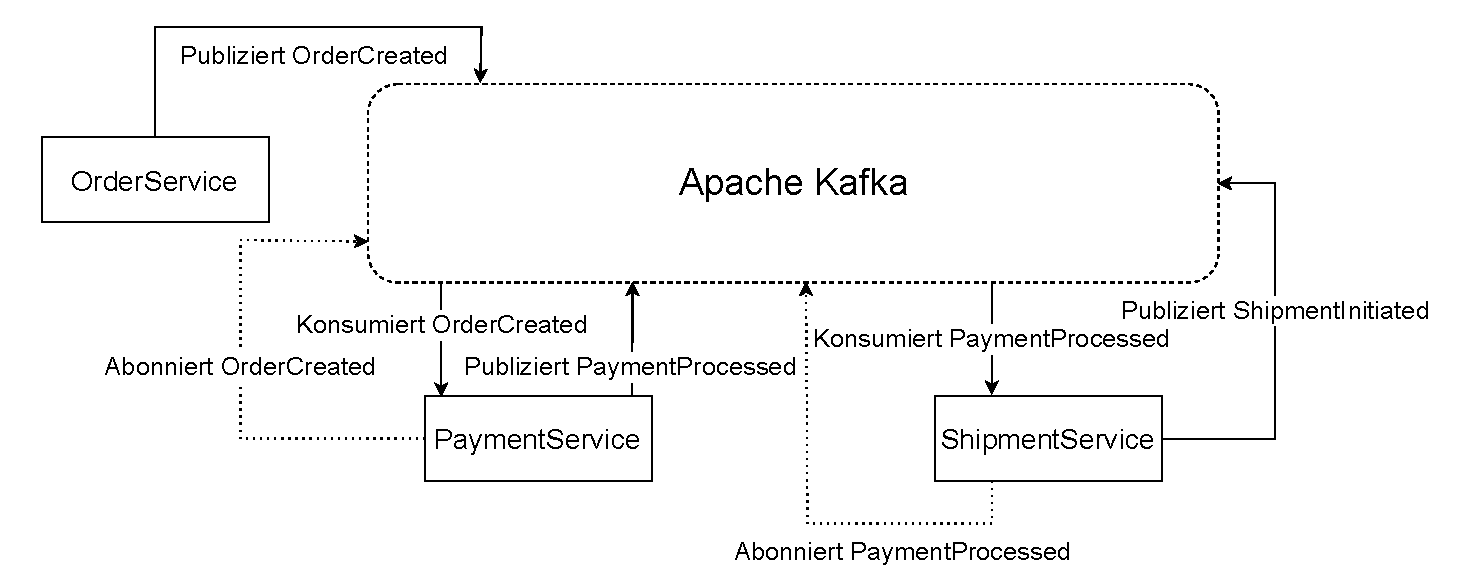
\includegraphics[width=\linewidth]{images/eda/eda-ecommerce.drawio}
  \caption{E-Commerce-Beispiel mit Event-Driven Architecture}
  \label{fig:edaecommerce}
\end{figure}
Wie Abbildung \ref{fig:edaecommerce} zeigt, sind alle drei Dienste Produzenten und Publisher, erzeugen also Events und veröffentlichen diese.
Die Dienste \texttt{PaymentService} und \texttt{ShipmentService} sind zudem Konsumenten,
sodass ersterer auf Events des Typs \texttt{OrderCreated} und zweiterer auf Events des Typs \texttt{ShipmentInitiated} reagiert.
Eine beispielhafte Implementierung des \texttt{PaymentService} mit Apache Kafka als Event-Broker ist im Anhang \ref{app:code:eda:paymentservice} zu finden.
Die vollständige Implementierung des E-Commerce-Beispiels ist bei GitHub \footnote{https://github.com/Beleg-6-EAP/demo-eda-ecommerce} zu finden.

Das Beispiel zeigt, dass die Event-Driven Architektur mit weiteren agilen Strukturen wie Microservices kombiniert werden kann, was die Agilität der Architektur weiter erhöht.
Die damit einhergehende Komplexität stellt teilweise hohe Anforderungen an die Entwickler.
Aufgrund der Asynchronität der Behandlung von Ereignissen ist die Testung des Systems meist schwer und die Fehlerbehandlung essentiell.
Mögliche Problemquellen schließen dabei unter anderem Event-Verlust, erhöhte Latenz und Inkonsistenz ein.
Die hohen Anforderungen an die Entwickler verlangen viel Vertrauen in jene, einer der zentralen Punkte des agilen Manifests \cite{agileManifesto}.
Insgesamt weist die Event-Driven Architecture also eine sehr hohe Agilität auf und ist damit besonders für moderne Software und ihre stetig wechselnden Anforderungen geeignet.

\section{Cloud-Native Architecture}
\label{sec:cloudnative}
Die Cloud-Native Architecture beruht auf der Annahme, dass die Infrastruktur in ständigem Wandel ist und die Auslagerung jener in die Cloud mehr Agilität schafft \cite{cloudNative}.
Als Cloud wird in diesem Fall die Infrastruktur eines oder mehrerer Cloud-Vendors bezeichnet.
Ein Cloud-Vendor bietet seine Infrastruktur und deren Verwaltung dabei gegen eine Gebühr an.
Unter anderem offeriert er:
\begin{itemize}
  \item Die globale Nutzung von Ressourcen durch Geo-Redundanz und somit starke Verteilung sowie hohe Verfügbarkeit von Software,
  \item dynamische Skalierung bereitgestellter Ressourcen basierend auf der Nachfrage von Software (Auto-Scaling),
  \item nutzungsbedingte Gebühren, sodass nur tatsächlich verwendete Ressourcen bezahlt werden (Pay-as-you-go),
  \item unterbrechungsfreie Updates von Software (Zero Downtime).
\end{itemize}

Als cloud-nativ wird hierbei all jene Software bezeichnet, welche explizit für die Cloud entwickelt wurde.
Grundsätzlich baut die cloud-native Architektur auf die in diesem Artikel bereits in Abschnitt \ref{sec:microservice} erklärte Microservice-Architektur und die
in Abschnitt \ref{sec:eda} erklärte Event-Driven Architecture auf.
Zusätzlich kommen sogenannte \textit{Fully Managed Cloud-Services} hinzu, was cloud-spezifische und vom Cloud-Vendor vollständig verwaltete Dienste sind.
Jene umfassen alle von Datenbanken über Message-Queues bis hin zu Serverless-Functions und viele mehr.
Charakterisiert werden diese durch die Eigenschaft, dass sich der Entwickler gänzlich auf die Business-Logik konzentrieren kann, da der Cloud-Provider
die vollständige Verwaltung der Infrastruktur übernimmt.
Zentral dabei ist der Aspekt der Containerisierung, bei welchem jede Komponente eines Systems in einen Container gepackt wird.
Der Cloud-Vendor kann die Gesamtheit der Container dann dynamisch orchestrieren und somit gezielt den Ressourcenverbrauch optimieren.

Im Folgenden greifen wir erneut das Beispiel E-Commerce aus der Einleitung auf und betrachten die Anpassung der in
Abschnitt \ref{sec:eda} angewendeten Event-Driven-Architecture auf die Cloud-Native Architecture mit Cloud-Vendor AWS\@.

Dabei ersetzen wir den dort verwendeten Broker durch eine \textit{Event-Bridge} \footnote{https://aws.amazon.com/de/eventbridge/, abgerufen am 06.01.2025}
- ein serverless Cloud-Service von AWS zum Routen von Ereignissen.
Weiter werden die drei Services für Aufgeben einer Bestellung, Bearbeitung der Bezahlung und Initiierung des Versands als \textit{Lambda} \footnote{https://aws.amazon.com/de/lambda/, abgerufen am 06.01.2025},
also Serverless-Function implementiert.
Abbildung \ref{fig:cloudnativeecommerce} stellt diese cloud-native Architektur dar.
Eine beispielhafte Implementierung des \texttt{ProcessPaymentLambda}s ist im Anhang \ref{app:code:cloudnative:paymentservice} und auf GitHub\footnote{https://github.com/Beleg-6-EAP/demo-cloud-native-ecommerce} zu finden.
\begin{figure}[!h]
  \centering
  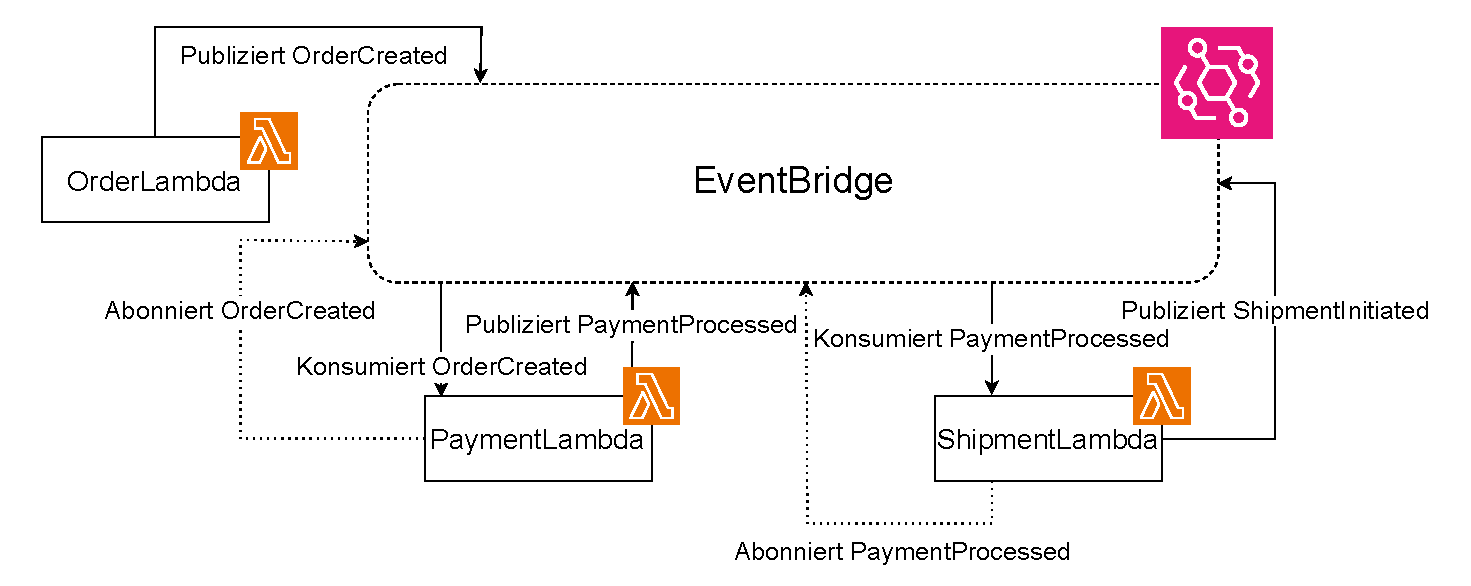
\includegraphics[width=\linewidth]{images/cloud-native/cloud-native-ecommerce.drawio}
  \caption{E-Commerce-Beispiel mit Cloud-Native Architecture}
  \label{fig:cloudnativeecommerce}
\end{figure}

Damit kombiniert die Cloud-Native Architecture die agilen Vorteile der Microservice- und Event-Driven Architecture.
Weiter ermöglichen die Cloud-Vendors nahtlose und einfache Möglichkeiten zur Auslieferung der Software,
wie beispielsweise Code-Deploy \footnote{https://aws.amazon.com/de/codedeploy/, abgerufen am 06.01.2024} bei AWS\@.
Die Option, allen Fokus von der Infrastruktur auf die Entwicklung zu legen, ermöglicht gemeinsam mit der einfachen Auslieferung kurze Iterationen in agilen Teams
und somit noch kürzere Zyklen in der Bereitstellung von Software.
Dabei ist besonders die Time-to-Market sehr gering, sodass Tech-Start-Ups häufig cloud-native Architekturen für ihre Software wählen. % TODO: Quelle!

Nicht zu vergessen ist zudem die extrem hohe Flexibilität der eingesetzten Ressourcen durch das Auto-Scaling.
Das damit verbundene Pay-as-you-go ermöglicht weiter auch finanzielle Agilität, wodurch zum Beispiel keine Vorab-Investitionen für Infrastruktur notwendig sind.
Jedoch ist zu betonen, dass aufgrund dessen auch Kostenrisiken durch möglicherweise unerwartete, extrem hohe Nachfrage der Software bestehen.
Ebenfalls nicht zu vernachlässigen ist die enge Bindung an den Cloud-Vendor durch Verwendung seiner spezifischen Cloud-Dienste.
Im Fall einer Migration zu einem anderen Cloud-Vendor könnten sowohl hohe Kosten beim vorherigen Cloud-Vendor, als auch Entwicklungskosten durch die notwendige
Anpassung der genutzten spezifischen Cloud-Dienste anfallen.
Obwohl das die Wahl des Cloud-Anbieters und der damit verbunden Entwicklung weniger agil macht, gilt die Cloud-Native Architecture besonders aufgrund der Auslagerung
der Infrastruktur als eine - und vermutlich die agilste Architektur für moderne Software.

\section{Microkernel Architecture}
\label{sec:microkernel}
Die Microkernel Architecture ist ein Architekturmuster, was sich durch Erweiterbarkeit, Flexibilität und vor allem Isolation der Funktionalitäten auszeichnet.
Wie in Abbildung~\ref{fig:microkernel} dargestellt, enthält ein Microkernel zwei wesentliche Komponenten: Den Kern der Anwendung,der die wichtigsten grundlegenden Funktionalitäten bereitstellt und Module oder auch Plugins,
die diesen Kern um Features erweitern~\cite[21-22]{architecturePatterns}.

\begin{figure}[!h]
  \centering
  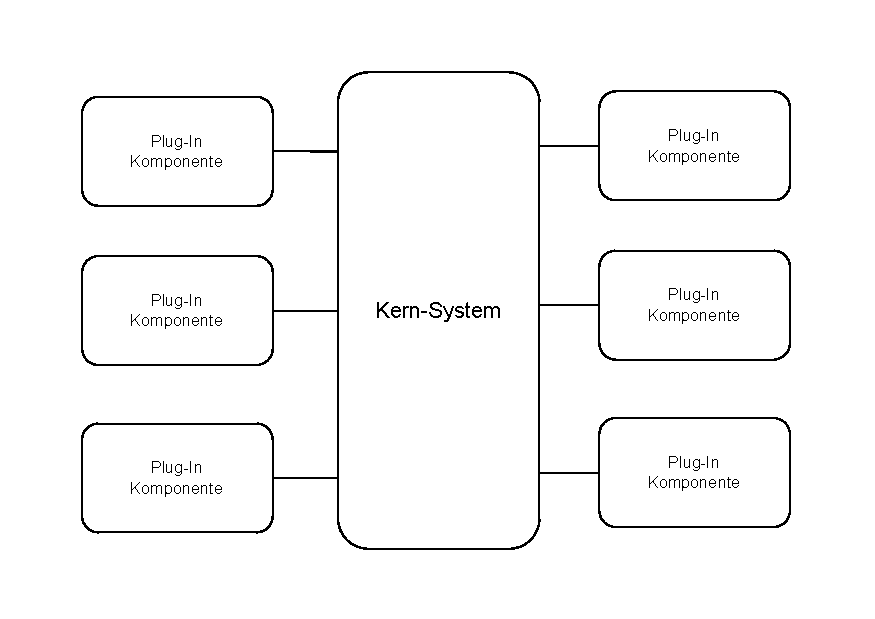
\includegraphics[width=\linewidth]{images/microkernel/microkernel}
  \caption{Aufbau einer Microkernel Architecture}
  \label{fig:microkernel}
\end{figure}

Der Kern der Anwendung implementiert dabei meist nur die minimalste Funktionalität, um die Anwendung oder das System lauffähig zu machen.
Alle weiteren Funktionalitäten werden in Modulen implementiert, die auf den Kern aufbauen.
Module sind meist unabhängig voneinander aufgebaut, es kann jedoch auch vorkommen, dass manche Module von anderen abhängig sind.
Best practice für die Entwicklung von Microkernel Architekturen ist es, die Kommunikation zwischen einzelnen Modulen so gering wie möglich zu halten, um Probleme durch Abhängigkeiten zu vermeiden.
Dadurch sind Module untereinander lose gekoppelt und können unabhängig voneinander entwickelt, getestet und deployed werden~\cite[22]{architecturePatterns}.

Die Plugins können über verschiedene Wege mit dem Kern verbunden werden.
Eine genaue Spezifikation zum Verbinden der Plugins mit dem Kern gibt es aber laut Architekturschema nicht, diese Entscheidung ist dem Entwickler überlassen und entsprechend der Anforderungen und Anwendungsumgebung zu treffen.
Unabhängig von der Art der Verbindung definiert der Kern die Schnittstellen, um Plugins anzubinden.
Diese Verbindung könnte dann beispielsweise über Web-Services, Messaging oder am einfachsten über direkte Objekt-Instanziierung innerhalb der gleichen Anwendung stattfinden~\cite[22-23]{architecturePatterns}.

Zwischen Plugins und Kern werden Verträge definiert, die die Kommunikation zwischen den beiden Komponenten regeln.
Diese Verträge können in Form von Interfaces, Klassen oder auch Datenstrukturen definiert werden.
Alle Plugins, müssen sich zwingend an die definierten Verträge halten, um mit dem Kern kommunizieren zu können.
Alternativ können auch Adapter verwendet werden, um bestehende Plugins an den Kern und die Verträge anzupassen, wodurch wiederrum die lose Kopplung der Komponenten verbessert wird.

Durch diesen Aufbau ergibt sich jedoch das Problem, dass der Kern jederzeit über Verfügbarkeit und Erreichbarkeit der Plugins informiert sein muss.
Um dieses Problem zu lösen, kann eine zentrale Plugin-Registry verwendet werden.
Diese Registry enthält alle aktuell verfügbaren Plugins sowie die dazugehörigen relevanten Informationen wie zum Beispiel Name des Service, Verträge, Verbindungsdetails, etc.
Der Kern der Anwendung kann dann zur Laufzeit auf diese Registry zugreifen und Plugins dynamisch laden~\cite[22]{architecturePatterns}.

Microkernel Architekturen können auch in andere Architekturmuster eingebettet werden, falls es nicht möglich sein sollte die gesamte Software in diesem Architekturmuster aufzubauen.
Vor allem Teile von Anwendungen, die stark erweiterbar sein müssen, eignen sich gut für die Verwendung der Microkernel Architektur.

Ein klarer Vorteil dieses Architekturmusters ist die schnelle Reaktionsfähigkeit auf äußere Änderungen, da Anpassungen aufgrund der losen Kopplung größtenteils nur in den isolierten Modulen vorgenommen werden.
Der Kern der Anwendung ist in den meisten Fällen schnell stabil und benötigt selten im Laufe der Entwicklung weitere Angleichungen.
Geänderte Module können je nach Implementierung auch zur Laufzeit geladen oder hinzugefügt werden, was mögliche Downtime von bereits ausgelieferter Software minimiert~\cite[25]{architecturePatterns}.

Ein Beispiel dafür stellt die Entwicklung von Betriebssystem-Kernels dar, die auch namensgebend für dieses Architekturmuster ist.
Deren Kern Komponenten sind in der Regel sehr stabil und implementieren vor allem grundlegende Funktionen wie Speicherverwaltung, Prozessverwaltung und I/O-Operationen.
Weitere low-level Funktionalitäten wie beispielsweise Geräte Treiber oder Dateisysteme werden als Module in den Kernel geladen und können bei Bedarf hinzugefügt oder entfernt werden, was vor allem für die Unterstützung neuer Hardware wichtig ist.

Auch Entwicklungsumgebungen in der Softwareentwicklung nutzen oft Microkernel Architekturen, um die Support für verschiedene Programmiersprachen und Frameworks zu ermöglichen.

Zwar bietet das Beispiel der E-Commerce Anwendung keinen klassischen Anwendungsfall für Microkernel Architekturen, jedoch kann die Verwendung von Microkernel Architekturen in Teilen der Anwendung trotzdem sinnvoll sein.
Sowohl Zahlungs- als auch Versandfunktionalitäten könnten, wie in Abbildung~\ref{fig:ecommerce-microkernel} dargestellt, in Module ausgelagert werden, um die Anwendung durch weitere Dienstleister erweitern zu können.

\begin{figure}[!h]
  \centering
  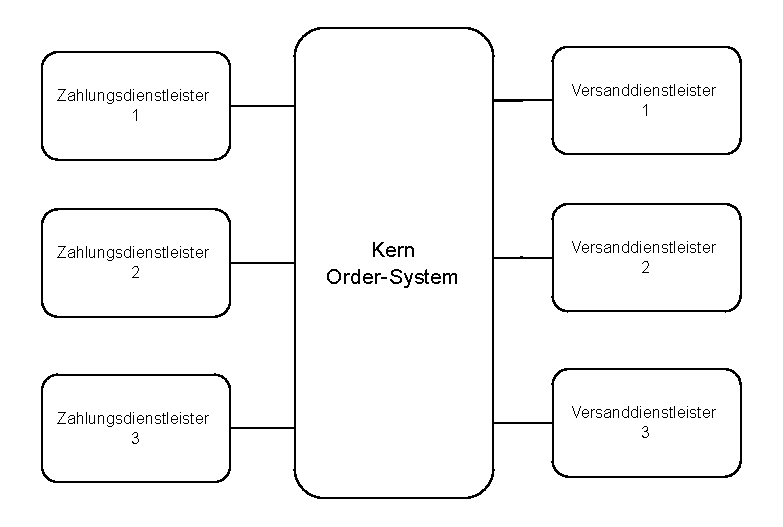
\includegraphics[width=\linewidth]{images/microkernel/ecommerce-microkernel}
  \caption{Aufbau der E-Commerce Anwendung mit Microkernel Architektur}
  \label{fig:ecommerce-microkernel}
\end{figure}

Logik zum Verarbeiten der Zahlungen und Versandinformationen wird dann in den Modulen implementiert, die auf den Kern der Anwendung aufbauen.
Dabei ist jedoch ein Großteil der Business-Logik im Kern der Anwendung enthalten, was nicht dem eigentlichen Gedanken der Microkernel Architektur entspricht.

Abgesehen davon erhöhen Microkernel Architekturen inhärent die Testbarkeit der Software, da Module nur lose Kopplung gekoppelt sind.
Jedes Modul kann unabhängig voneinander getestet werden und fehlende Module durch Stubs ersetzt werden, wodurch sich während der Entwicklung auf einzelne Module isoliert konzentriert werden kann~\cite[26]{architecturePatterns}.
Weiterhin können Verhaltensweisen von anderen Modulen durch Mocks simuliert werden, um Testzustände zu erzeugen und das Verhalten der Anwendung zu verifizieren.
In Agilen Umgebungen, in denen das Testen von Software eine wichtige Rolle spielt, ist die Verwendung von Microkernel Architekturen daher besonders sinnvoll.

Eine Herausforderung bei der Verwendung von Microkernel Architekturen kann jedoch der Entwurf der Kern-Komponente darstellen.
Da alle anderen Module auf den Kern aufbauen, muss dieser sehr sorgfältig und stabil entwickelt werden, um die Funktionalität der gesamten Anwendung zu gewährleisten.
Diese Rolle sollten vor allem erfahrene Entwickler übernehmen, da sich Design-Fehler der Kern-Komponente oder Verträge negativ auf die Entwicklung der Module auswirken können.
Sollte der Kern der Anwendung angepasst werden, so müssen tendenziell auch alle Module überprüft oder aktualisiert werden, was zu erheblich erhöhten Entwicklungszeiten führen kann und zuvor gewonnene Vorteile der Microkernel Architektur zunichte macht.

Aufgrund der initial hohen Komplexität, die mit der Entwicklung des Kerns einhergeht, stellt die Microkernel Architektur nicht die beste Wahl dar, wenn es darum geht schnell eine erste Version der Software auf den Markt zu bekommen.
Die wesentlichen Vorteile, die die Microkernel Architektur bietet, zeigen sich erst im späteren Verlauf der Entwicklung, wenn die Anwendung erweitert werden muss.
Sowohl Iterationen als auch Auslieferungszeiten sind dann sehr kurz, da Module unabhängig voneinander entwickelt werden und die Anwendung schnell an neue Anforderungen angepasst werden kann.
Diese Vorteile können die Architektur in ausgewählten Anwendungsfällen sehr geeignet für agile Entwicklungsumgebungen machen.

\section{Zusammenfassung und Ausblick}
\label{sec:summary}
In dieser Arbeit wurden verschiedene Enterprise-Architektur-Muster untersucht und deren Eignung für moderne Geschäftsprozesse bewertet.
Dabei wurde festgestellt, dass die Agilität im Entwicklungsprozess maßgeblich durch die Wahl des Architekturmusters beeinflusst wird.

Die monolithische Architektur zeichnet sich durch die Verwendung einer einzigen Komponente aus, die alle Funktionalitäten der Anwendung bereitstellt.
Modular monolithische Architekturen bauen auf dieser Idee auf, indem sie die monolithische Anwendung in Module unterteilen, um die Wartbarkeit zu verbessern.
SOA teilt die Anwendung in grobe Dienste auf, was die Wiederverwendung von Funktionalitäten ermöglicht.
Microservices verbessern die Skalierbarkeit und Wartbarkeit von SOA, indem sie die Dienste in noch kleinere, isolierte Komponenten aufteilen, die nur über standardisierte Schnittstellen kommunizieren.
Das Alleinstellungsmerkmal von Event-Driven Architekturen sind die asynchronen Reaktionen auf Ereignisse, wodurch die Anwendung sehr flexibel und skalierbar wird.
Cloud-native Architekturen lagern die Verwaltung der Infrastruktur an Cloud-Anbieter aus, sodass sich in der Entwicklung auf die Business-Logik konzentriert werden kann.
Als Architektur für besonders erweiterbare Anwendungen lässt sich die Microkernel-Architektur verwenden, die die Anwendung auf einen Kern mit wenig Funktionalität und Plugins mit Business-Logik auftrennt.

Eine Bewertung der Architekturen anhand von Agilen Kriterien ist in Tabelle~\ref{tab:overview} dargestellt.

\begin{table}[H]
    \scalebox{0.7}{
        \begin{tabular}{|l|c|c|c|c|c|c|c|c|}
            \hline
            & \rot{Monolith}     & \rot{Mod. Monol.}  & \rot{SOA} & \rot{Microservices} & \rot{Layered} & \rot{EDA} & \rot{Cloud-Native}  & \rot{Microkernel} \\
            \hline
            Time-To-Market         & \cmark\cmark\cmark & \cmark\cmark\cmark & 0         & \xmark              & ?             & \xmark             & \cmark\cmark & \xmark\xmark\xmark \\
            \hline
            Skalierbarkeit         & \xmark\xmark\xmark & \xmark\xmark\xmark & \xmark    & \cmark\cmark\cmark  & ? & \cmark\cmark\cmark & \cmark\cmark\cmark & 0 \\
            \hline
            Kostenflexibilität     & \xmark\xmark       & \xmark\xmark       & \xmark    & \cmark              & ?             & \cmark             & \cmark\cmark\cmark & \xmark \\
            \hline
            Anforderungsänderungen & \xmark\xmark\xmark & \xmark\xmark       & \cmark    & \cmark\cmark\cmark & \cmark\cmark & \cmark\cmark\cmark & \cmark\cmark\cmark & \cmark\cmark \\
            \hline
            Erweiterbarkeit        & \xmark\xmark\xmark & \xmark\xmark       & 0         & \cmark\cmark        & \cmark\cmark  & \cmark\cmark & \cmark\cmark & \cmark\cmark\cmark \\
            \hline
            Auslieferung           & \xmark\xmark\xmark & \xmark\xmark\xmark & \cmark    & \cmark\cmark        & \cmark        & \cmark\cmark & \cmark\cmark\cmark & \cmark\cmark \\
            \hline
        \end{tabular}}
    \caption{Vergleich der Architekturmuster}
    \label{tab:overview}
\end{table}

Auffallend ist zum einen, dass monolithische Anwendungen zwar die beste Time-To-Market haben, den anderen Architekturmustern jedoch in allen anderen Vergleichspunkten unterlegen.
Die Architekturen mit der besten Skalierbarkeit zeichnen sich durch die starke Isolation von Komponenten aus und sind hier Microservices, Event-Driven und Cloud-Native Architekturen.
Die einzige Architektur, die eine hohe Flexibilität bei den Kosten aufweist, ist die Cloud-Native Architektur, da nur die tatsächlich genutzten Ressourcen bezahlt werden.
Auf Änderungen in den Anforderungen können alle modernen Architekturen sehr gut reagieren.
Die beste Erweiterbarkeit weist die Microkernel Architektur auf, da die Business-Logik größtenteils durch Plugins realisiert wird.
Betrachten wir die Auslieferung von Software, so schneiden traditionelle Architekturen hier am schlechtesten ab, da sie nur im Ganzen ausgetauscht werden können.
Moderne Architekturen, insbesondere Microservices, Event-Driven und Cloud-Native Architekturen, können Software in kleinen Teilen ausliefern und so schneller auf Änderungen der Anforderungen reagieren.
Die Layered Architektur ist hier teilweise schwer einzuordnen, da sie meistens mit anderen Architekturmustern kombiniert wird, die einen wesentlichen Einfluss auf Time-To-Market, Skalierbarkeit und Kosten haben.

Betrachten wir das E-Commerce-Beispiel und die anfangs gestellten Anforderungen, so zeigt sich, dass die Cloud-Native Architektur in diesem Fall die beste Wahl darstellt.
Es kann schnell auf technische Änderungen reagiert werden, die in produktiv-Umgebungen einfach ausgerollt werden können.
Wachsender Traffic, der später auftreten könnte, kann durch Auto-Scaling einfach bewältigt werden.
Entwickler, die sich auf den Aufbau der Infrastruktur konzentrieren, sind nicht nötig und können sich an der Entwicklung der Business-Logik beteiligen.
Die Kosten sind flexibel und nur abhängig von der tatsächlichen Nutzung der Ressourcen, was vor allem am Anfang bei geringen Nutzerzahlen Kosten spart.
Aufgrund der geringen Time-To-Market ist es außerdem möglich, einen MVP schnell auf den Markt zu bringen und diesen dann iterativ zu verbessern.

Unabhängig davon gilt jedoch, dass es kein universell bestes Architekturmuster gibt.
Die Wahl der Architektur muss den spezifischen Anforderungen eines Projekts angepasst sein und besteht meist aus einer Kombination mehrerer EA-Muster.

Damit bleibt die Frage offen, wie hybride Architekturen aussehen könnten, die Elemente aus verschiedenen EA-Architekturen kombinieren, um alle agilen Anforderung bestmöglich zu erfüllen.

\bibliographystyle{ACM-Reference-Format}
\bibliography{main}

\appendix

\section{Code-Beispiele}

\subsection{Monolithic Architecture}
\label{app:code:monolithic:paymentservice}
\begin{listing}[H]
  \tiny
  \inputminted[linenos=true]{java}{code/monolithic/PaymentService.java}
  \caption{Service-Implementierung des \texttt{PaymentService} in Java Spring Boot 3.4.1}
\end{listing}

\subsection{Modular Monolithic Architecture}
\label{app:code:modular:orderservice}
\begin{listing}[H]
  \tiny
  \inputminted[linenos=true]{java}{code/modulithic/OrderServiceImpl.java}
  \caption{Service-Implementierung des \texttt{OrderService} in Java Spring Boot 3.4.1}
\end{listing}

\subsection{Event-Driven Architecture}
\label{app:code:eda:paymentservice}
\begin{listing}[H]
  \tiny
  \inputminted[linenos=true]{java}{code/eda/PaymentService.java}
  \caption{Service-Implementierung des \texttt{PaymentService} in Java Spring Boot 3.4.1 mit Apache Kafka als Event-Broker}
\end{listing}

\subsection{Cloud-native Architecture}
\label{app:code:cloudnative:paymentservice}
\begin{listing}[H]
  \tiny
  \inputminted[linenos=true]{haskell}{code/cloud/PaymentService.hs}
  \caption{Implementierung des \texttt{ProcessPaymentLambda}s in Haskell}
\end{listing}

\subsection{Service-oriented Architecture}
\label{app:code:soa:registry}
\begin{listing}[H]
  \tiny
  \inputminted[linenos=true]{ruby}{code/soa/service_registry.rb}
  \caption{Implementierung der \texttt{ServiceRegistry} in Ruby on Rails}
\end{listing}

\section{Übungsaufgaben}
\subsection{Übungsaufgabe 1}
Das E-Commerce-Beispiel aus der Einleitung soll um Nutzer-Authentifizierung erweitert werden.
Sie haben sich zuvor für eine Microservice-Architektur entschieden und die in der Einleitung genannten Anforderungen implementiert.
Die Authentifizierung wird in verschiedenen Komponenten benötigt.
Erläutern Sie, wie Sie die Authentifizierung in die Architektur integrieren.

\subsection{Übungsaufgabe 2}
Das E-Commerce-Beispiel aus der Einleitung soll um Logging erweitert werden.
Sie haben sich zuvor für eine cloud-native Event-Driven-Architektur entschieden und die in der Einleitung genannten Anforderungen implementiert.
Das Logging wird in verschiedenen Komponenten benötigt.
Erläutern Sie, wie Sie das Logging in die Architektur integrieren.
Bedenken Sie dabei, dass Logs aus verschiedenen Komponenten möglicherweise zur Auswertung zusammengeführt werden müssen und somit die Reihenfolge von Logs relevant ist.

\subsection{Übungsaufgabe 3}
Das E-Commerce-Beispiel aus der Einleitung soll um ein E-Mail-Notifikationssystem erweitert werden.
Dieses soll Nutzern E-Mails bei jeder Statusänderung einer ihrer Bestellungen zustellen.
Untersuchen Sie für alle in diesem Papier betrachteten Architekturen, wie das E-Mail-Notifikationssystem in die bestehende Architektur integriert werden kann
und welche Vor- und Nachteile diese Integration in die jeweilige Architektur mit sich bringt.
Für welche der Architekturen ist die Integration des E-Mail-Notifikationssystems am einfachsten?

\end{document}
\endinput
